\documentclass[aspectratio=169]{beamer}

\usepackage[utf8]{inputenc}
\usepackage[T1]{fontenc}
\usepackage{lmodern}
\usepackage{booktabs}
\usepackage{tabularx}
\usepackage{tikz}
\usepackage{xcolor}
\usepackage{hyperref}
\usetikzlibrary{positioning,arrows.meta}

\definecolor{accent1}{HTML}{0F766E}
\definecolor{accent2}{HTML}{99F6E4}
\definecolor{accent3}{HTML}{F59E0B}
\definecolor{accent4}{HTML}{134E4A}
\definecolor{paper}{HTML}{F7FEFC}
\definecolor{ink}{HTML}{1F2937}
\definecolor{softgray}{HTML}{F3F4F6}

\hypersetup{
  colorlinks=true,
  urlcolor=accent1,
  linkcolor=accent4
}

\setbeamertemplate{navigation symbols}{}
\setbeamercolor{normal text}{fg=ink,bg=white}
\setbeamercolor{frametitle}{fg=ink,bg=white}
\setbeamertemplate{itemize item}{\color{accent1}$\blacktriangleright$}
\setbeamertemplate{enumerate item}{\color{accent1}\insertenumlabel.}
\setbeamerfont{frametitle}{series=\bfseries,size=\Large}

\newcommand{\LocalLink}[2]{\href{run:#1}{#2}}
\newcommand{\WebLink}[2]{\href{#1}{#2}}
\newcolumntype{Y}{>{\raggedright\arraybackslash}X}

\title{Teaching Students to Use AI as a Learning Partner}
\subtitle{MagicSchool materials, process, and transcript-based learning}
\author{Pine Brook IGNITE}
\date{Spring 2026}

\begin{document}

\begin{frame}[plain]
\begin{tikzpicture}[remember picture,overlay]
\fill[paper] (current page.south west) rectangle (current page.north east);
\fill[accent1!10] (0.25,0.4) rectangle (13.05,7.0);
\draw[line width=7pt, color=accent3] (0.55,6.75) -- (12.75,6.75);
\draw[line width=7pt, color=accent2] (0.55,0.65) -- (12.75,0.65);
\end{tikzpicture}
\vspace{0.55cm}
{\huge\bfseries Teaching Students to Use AI as a Learning Partner\par}
\vspace{0.25cm}
{\Large\color{accent4} Materials, process, and what we learned from classroom evidence\par}
\vspace{0.45cm}
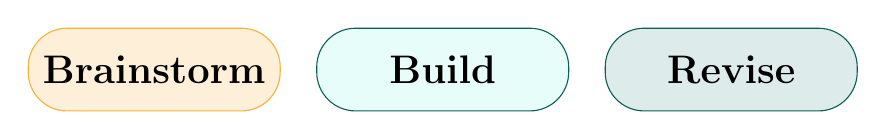
\begin{tikzpicture}[node distance=0.45cm]
\node[rounded corners=14pt, fill=accent3!16, draw=accent3!80, minimum width=3.2cm, minimum height=1.05cm, align=center] (a) {\Large\bfseries Brainstorm};
\node[rounded corners=14pt, fill=accent2!24, draw=accent1!80!black, minimum width=3.2cm, minimum height=1.05cm, align=center, right=of a] (b) {\Large\bfseries Build};
\node[rounded corners=14pt, fill=accent1!14, draw=accent1!80!black, minimum width=3.2cm, minimum height=1.05cm, align=center, right=of b] (c) {\Large\bfseries Revise};
\end{tikzpicture}
\vspace{0.35cm}
\begin{block}{Core idea}
\large AI helps students think, plan, check, and revise. Students stay responsible for choices, voice, and final work.
\end{block}
\end{frame}

\begin{frame}
\frametitle{Module Context}
\begin{block}{Three-session sequence}
\begin{enumerate}
\large
\item \textbf{Lesson 1: Brainstorm and Plan} -- choose a topic, check the CS connection, generate a high-level guide.
\item \textbf{Lesson 2: Build Step by Step} -- use the guide to build project sections with AI support.
\item \textbf{Lesson 3: Revise and Validate} -- finish, compare to the plan, revise, and explain AI use.
\end{enumerate}
\end{block}
\vspace{0.15cm}
\begin{block}{Product menu}
\large Slideshow, poster/one-pager, booklet, or simple site.
\end{block}
\end{frame}

\begin{frame}
\frametitle{Materials Used}
\small
\begin{tabularx}{\textwidth}{@{}p{3.1cm}Yp{3.4cm}@{}}
\toprule
\textbf{Material} & \textbf{What it does} & \textbf{Link} \\
\midrule
Main lesson packet & Defines the full 3-session AI partner project, goals, norms, product menu, and assessment frame. & \LocalLink{magicschool-student-choice-ai-partner-project.pdf}{packet PDF} \\
Lesson 1 folder & Holds setup, student directions, prompt cards, rubric, exit ticket, and slides for brainstorming. & \LocalLink{lesson1/}{lesson1 folder} \\
Lesson 2 folder & Holds setup, student directions, rubric, exit ticket, and slides for building from the guide. & \LocalLink{lesson2/}{lesson2 folder} \\
Transcript anchor & Shows how Lesson 1 went in class and what needed adjustment for Lesson 2. & \LocalLink{../../../../transcripts/2026-04-10\%20Lecture_\%20AI\%20Project\%20Brainstorming\%20and\%20Planning-transcript.txt}{Apr. 10 transcript} \\
Official references & Ground safety, AI literacy, CS standards, and inclusion choices. & \LocalLink{magicschool-student-choice-ai-partner-project.bib}{bibliography} \\
\bottomrule
\end{tabularx}
\end{frame}

\begin{frame}
\frametitle{Official Reference Anchors}
\begin{itemize}
\large
\item \WebLink{https://www.magicschool.ai/magicstudent}{MagicStudent}: teacher-managed student AI access.
\item \WebLink{https://www.magicschool.ai/privacy}{MagicSchool privacy and security}: safe, monitored classroom use.
\item \WebLink{https://iste.org/areas-of-focus/ai-in-education}{ISTE AI in Education}: AI literacy and responsible classroom integration.
\item \WebLink{https://unesdoc.unesco.org/ark:/48223/pf0000386693}{UNESCO generative AI guidance}: human agency, age-appropriate use, and checking AI output.
\item \WebLink{https://csteachers.org/k12standards/interactive/}{CSTA K-12 Standards}: CS-aligned problem solving, tools, and responsible computing.
\end{itemize}
\end{frame}

\begin{frame}
\frametitle{AI Partner Mini-Framework}
\begin{center}
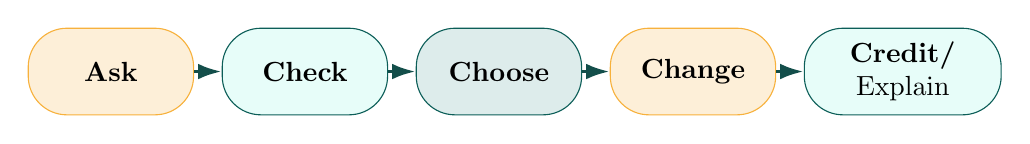
\begin{tikzpicture}[node distance=0.35cm]
\node[rounded corners=14pt, fill=accent3!16, draw=accent3!80, minimum width=2.1cm, minimum height=1.1cm, align=center] (ask) {\bfseries Ask};
\node[rounded corners=14pt, fill=accent2!24, draw=accent1!80!black, minimum width=2.1cm, minimum height=1.1cm, align=center, right=of ask] (check) {\bfseries Check};
\node[rounded corners=14pt, fill=accent1!14, draw=accent1!80!black, minimum width=2.1cm, minimum height=1.1cm, align=center, right=of check] (choose) {\bfseries Choose};
\node[rounded corners=14pt, fill=accent3!16, draw=accent3!80, minimum width=2.1cm, minimum height=1.1cm, align=center, right=of choose] (change) {\bfseries Change};
\node[rounded corners=14pt, fill=accent2!24, draw=accent1!80!black, minimum width=2.5cm, minimum height=1.1cm, align=center, right=of change] (credit) {\bfseries Credit/\\Explain};
\draw[-{Latex[length=3mm,width=2mm]}, line width=1.3pt, color=accent4] (ask) -- (check);
\draw[-{Latex[length=3mm,width=2mm]}, line width=1.3pt, color=accent4] (check) -- (choose);
\draw[-{Latex[length=3mm,width=2mm]}, line width=1.3pt, color=accent4] (choose) -- (change);
\draw[-{Latex[length=3mm,width=2mm]}, line width=1.3pt, color=accent4] (change) -- (credit);
\end{tikzpicture}
\end{center}
\vspace{0.25cm}
\begin{block}{Why it matters}
\large The routine makes AI use observable: students ask for help, check the response, choose what fits, change it, and explain their own decision.
\end{block}
\end{frame}

\begin{frame}
\frametitle{Lesson 1: Brainstorm and Plan}
\begin{columns}[T,totalwidth=\textwidth]
\column{0.48\textwidth}
\begin{block}{Goal}
\large Students leave with a topic, CS connection, product choice, and high-level guide.
\end{block}
\begin{block}{Tool flow}
\large \textbf{Idea Generator first}: generate CS-connected topic ideas.\\
\textbf{AI Assistant second}: check, narrow, and organize one topic.
\end{block}
\column{0.48\textwidth}
\begin{block}{Student process}
\begin{enumerate}
\large
\item Pick an interest.
\item Generate possible CS topics.
\item Choose one manageable topic.
\item Check CS fit.
\item Generate a guide with 3--5 parts.
\end{enumerate}
\end{block}
\end{columns}
\end{frame}

\begin{frame}
\frametitle{Lesson 1 Materials}
\small
\begin{tabularx}{\textwidth}{@{}p{3.2cm}Yp{3.1cm}@{}}
\toprule
\textbf{Material} & \textbf{Purpose} & \textbf{Link} \\
\midrule
AI setup & Teacher-facing configuration and tool roles for Idea Generator and AI Assistant. & \LocalLink{lesson1/lesson1-ai_setup.md}{setup} \\
AI directions & Student-facing workflow, approved prompts, and copying/checking rule. & \LocalLink{lesson1/lesson1-ai_directions.md}{directions} \\
Prompt cards & Copy-friendly prompt page for student access. & \LocalLink{lesson1/lesson1-prompt-cards-copy.html}{prompt cards} \\
Student slides & Classroom scaffolding for mission, rules, tool separation, workflow, and prompts. & \LocalLink{lesson1/lesson1-brainstorm-and-plan-slides.pdf}{slides PDF} \\
Rubric + exit ticket & Captures topic ownership, CS connection, planning with AI, safety, and readiness. & \LocalLink{lesson1/lesson1-rubric.md}{rubric} / \LocalLink{lesson1/lesson1-exit_ticket.md}{exit ticket} \\
\bottomrule
\end{tabularx}
\end{frame}

\begin{frame}
\frametitle{What the Transcript Showed for Lesson 1}
\begin{block}{Classroom observations from April 10, 2026}
\begin{itemize}
\large
\item Students needed explicit support for Google Classroom, duplicate tabs, MagicSchool login, and tool navigation.
\item Prompt copying had to be modeled slowly: select, copy, paste, replace the blank, then submit.
\item Student interests like space, soccer, animals, games, and cats were useful entry points.
\item The CS connection had to stay visible so topics did not become general-interest projects.
\item Many students reached a topic or project idea, but not all completed the full guide.
\end{itemize}
\end{block}
\end{frame}

\begin{frame}
\frametitle{Transcript-Based Adjustment}
\begin{columns}[T,totalwidth=\textwidth]
\column{0.48\textwidth}
\begin{block}{What worked}
\begin{itemize}
\large
\item Clear tool separation helped.
\item Copyable prompts reduced typing load.
\item Student choice increased engagement.
\item Teacher modeling made AI use safer.
\end{itemize}
\end{block}
\column{0.48\textwidth}
\begin{block}{What needed improvement}
\begin{itemize}
\large
\item Login and tab routines took real time.
\item Some students needed help choosing from AI output.
\item Lesson 2 needed a recovery checkpoint before building.
\item Success criteria needed to remain visible during work time.
\end{itemize}
\end{block}
\end{columns}
\end{frame}

\begin{frame}
\frametitle{Lesson 2: Build Step by Step}
\begin{columns}[T,totalwidth=\textwidth]
\column{0.48\textwidth}
\begin{block}{Goal}
\large Students use their topic and guide to build project sections, not restart brainstorming.
\end{block}
\begin{block}{Tool flow}
\large \textbf{AI Assistant}: recover/clarify/expand one guide part.\\
\textbf{Project tool}: build the actual slideshow, poster, booklet, or site.
\end{block}
\column{0.48\textwidth}
\begin{block}{Student process}
\begin{enumerate}
\large
\item Recover topic and guide.
\item Build Part 1.
\item Build Part 2.
\item Build Part 3.
\item Check against guide and CS goal.
\end{enumerate}
\end{block}
\end{columns}
\end{frame}

\begin{frame}
\frametitle{Lesson 2 Materials}
\small
\begin{tabularx}{\textwidth}{@{}p{3.2cm}Yp{3.1cm}@{}}
\toprule
\textbf{Material} & \textbf{Purpose} & \textbf{Link} \\
\midrule
AI setup & Teacher-facing setup for a single bounded AI tool and project-building workflow. & \LocalLink{lesson2/lesson2-ai_setup.md}{setup} \\
AI directions & Student-facing directions for using AI as a build partner. & \LocalLink{lesson2/lesson2-ai_directions.md}{directions} \\
Student slides & Recovery checkpoint, tool split, workflow, prompts, worked example, and midpoint check. & \LocalLink{lesson2/lesson2-build-and-execute-slides.pdf}{slides PDF} \\
Rubric & Checkpoint rubric for using the plan, step-by-step execution, CS accuracy, safe AI use, and Lesson 3 readiness. & \LocalLink{lesson2/lesson2-rubric.md}{rubric} \\
Exit ticket & Captures what students built, how AI helped, what they changed, and next steps. & \LocalLink{lesson2/lesson2-exit_ticket.md}{exit ticket} \\
\bottomrule
\end{tabularx}
\end{frame}

\begin{frame}
\frametitle{Why Lesson 2 Starts With Recovery}
\begin{block}{Instructional reason}
\large The transcript showed that Lesson 1 produced strong engagement and many project ideas, but the full guide was uneven across students.
\end{block}
\vspace{0.1cm}
\begin{block}{Lesson 2 response}
\begin{itemize}
\large
\item Confirm or rebuild topic, product type, CS connection, and guide.
\item Move quickly from recovery into building.
\item Use AI Assistant only for one section at a time.
\item Keep the project tool as the place where the real work is built.
\end{itemize}
\end{block}
\end{frame}

\begin{frame}
\frametitle{Student Workflow Across the Module}
\begin{center}
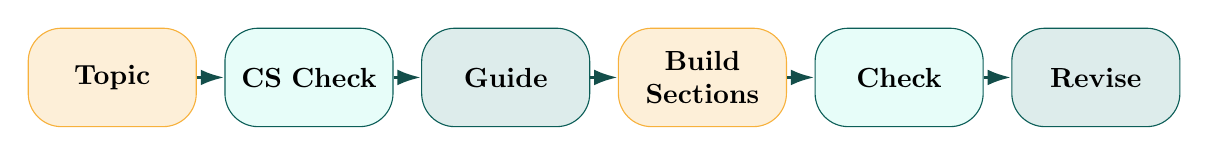
\begin{tikzpicture}[node distance=0.35cm]
\node[rounded corners=12pt, fill=accent3!16, draw=accent3!80, text width=1.9cm, minimum height=1.25cm, align=center] (a) {\bfseries Topic};
\node[rounded corners=12pt, fill=accent2!24, draw=accent1!80!black, text width=1.9cm, minimum height=1.25cm, align=center, right=of a] (b) {\bfseries CS Check};
\node[rounded corners=12pt, fill=accent1!14, draw=accent1!80!black, text width=1.9cm, minimum height=1.25cm, align=center, right=of b] (c) {\bfseries Guide};
\node[rounded corners=12pt, fill=accent3!16, draw=accent3!80, text width=1.9cm, minimum height=1.25cm, align=center, right=of c] (d) {\bfseries Build Sections};
\node[rounded corners=12pt, fill=accent2!24, draw=accent1!80!black, text width=1.9cm, minimum height=1.25cm, align=center, right=of d] (e) {\bfseries Check};
\node[rounded corners=12pt, fill=accent1!14, draw=accent1!80!black, text width=1.9cm, minimum height=1.25cm, align=center, right=of e] (f) {\bfseries Revise};
\draw[-{Latex[length=3mm,width=2mm]}, line width=1.2pt, color=accent4] (a) -- (b);
\draw[-{Latex[length=3mm,width=2mm]}, line width=1.2pt, color=accent4] (b) -- (c);
\draw[-{Latex[length=3mm,width=2mm]}, line width=1.2pt, color=accent4] (c) -- (d);
\draw[-{Latex[length=3mm,width=2mm]}, line width=1.2pt, color=accent4] (d) -- (e);
\draw[-{Latex[length=3mm,width=2mm]}, line width=1.2pt, color=accent4] (e) -- (f);
\end{tikzpicture}
\end{center}
\vspace{0.25cm}
\begin{block}{Teacher move}
\large Keep students moving from AI conversation into visible student work.
\end{block}
\end{frame}

\begin{frame}
\frametitle{CS Standards and Responsible AI}
\begin{columns}[T,totalwidth=\textwidth]
\column{0.48\textwidth}
\begin{block}{CS learning}
\begin{itemize}
\large
\item Use digital tools for a defined purpose.
\item Break a project into smaller parts.
\item Evaluate output from a computing system.
\item Organize information into a plan.
\item Communicate a digital product to an audience.
\end{itemize}
\end{block}
\column{0.48\textwidth}
\begin{block}{Responsible AI learning}
\begin{itemize}
\large
\item No private information in prompts.
\item AI output can be wrong.
\item Students choose what to keep or change.
\item Final work must show student voice.
\item Teacher monitors classroom AI use.
\end{itemize}
\end{block}
\end{columns}
\end{frame}

\begin{frame}
\frametitle{Inclusive Strategies}
\begin{itemize}
\large
\item Visual prompt frames and projected workflows reduce working-memory load.
\item Copyable prompts reduce typing and spelling barriers.
\item Students can talk, draw, point, or rehearse before typing.
\item Partner roles support reading directions and checking ideas.
\item Chunked checkpoints make progress visible.
\item Exit tickets capture learning even when the final product is not finished.
\end{itemize}
\end{frame}

\begin{frame}
\frametitle{What We Learned}
\begin{block}{Instructional takeaways}
\begin{itemize}
\large
\item AI lessons need as much tool-routine scaffolding as content scaffolding.
\item Prompt access matters: students need fast ways to copy, paste, and replace blanks.
\item Student choice works best when bounded by a clear CS connection.
\item Lesson 2 should not assume Lesson 1 ended perfectly; recovery is part of good design.
\item Assessment should capture student decisions, not just AI output.
\end{itemize}
\end{block}
\end{frame}

\begin{frame}
\frametitle{Closing Frame}
\begin{center}
{\huge\bfseries AI is the partner.\\[0.15cm] Students are the thinkers.}
\end{center}
\vspace{0.35cm}
\begin{block}{What to look for in the materials}
\large The strongest evidence of learning is when students can explain what they asked, what they checked, what they kept, what they changed, and why their project still meets the goal.
\end{block}
\end{frame}

\end{document}
